%!TEX root = ./workbook-2011.tex

\section{Vector Mathematics in R}

As you saw last week R vectors support basic arithmetic operations that
correspond to the same operations on geometric vectors. For example:
%
\begin{R}
> x <- 1:15
> y <- 10:24
> x
 [1]  1  2  3  4  5  6  7  8  9 10 11 12 13 14 15
> y
 [1] 10 11 12 13 14 15 16 17 18 19 20 21 22 23 24

> x + y             # vector addition
 [1] 11 13 15 17 19 21 23 25 27 29 31 33 35 37 39
> x - y             # vector subtraction
 [1] -9 -9 -9 -9 -9 -9 -9 -9 -9 -9 -9 -9 -9 -9 -9
> x * 3             # multiplication by a scalar
 [1]  3  6  9 12 15 18 21 24 27 30 33 36 39 42 45
\end{R}
%
R also has an operator for the dot product, denoted \lstinline!%*%!.
This operator also designates matrix multiplication, which we will
discuss next week. By default this operator returns an object of the R
matrix class. If you want a scalar (or the R equivalent of a scalar,
i.e.~a vector of length 1) you need to use the \lstinline!drop()!
function.

\begin{R}
> z <- x %*% x
> class(z)      # note use of class() function
[1] "matrix"
> z
     [,1]
[1,] 1240
> drop(z)
[1] 1240
\end{R}

In lecture we saw that many useful geometric properties of vectors could be expressed in the form of dot products. Let's start with some two-dimensional vectors where the geometry is  easy to visualize:

\begin{R}
> a <- c(1, 0) # the point (1,0)
> b <- c(0, 1) # the point (0,1)
\end{R}
%
Now let's draw our vectors:
%
\begin{R}
# create empty plot w/specified x- and y- limits
# the 'asp=1' argument maintains the scaling of the x- and y-axes
# so that units are equivalent for both axes (i.e. squares remain squares)
> plot(c(-2,2),c(-1,2),type='n', asp=1)

# draw an arrow from origin (0,0) to x,y coordinates of vector "a"
# the length argument changes the size of the arrowhead
# use the R help to read more about the arrows function
> arrows(0, 0, a[1], a[2], length=0.1)

# and now for the vector "b"
> arrows(0, 0, b[1], b[2], length=0.1)
\end{R}
%
You should now have a figure that looks like the one below:
\begin{figure}[htbp]
\centering
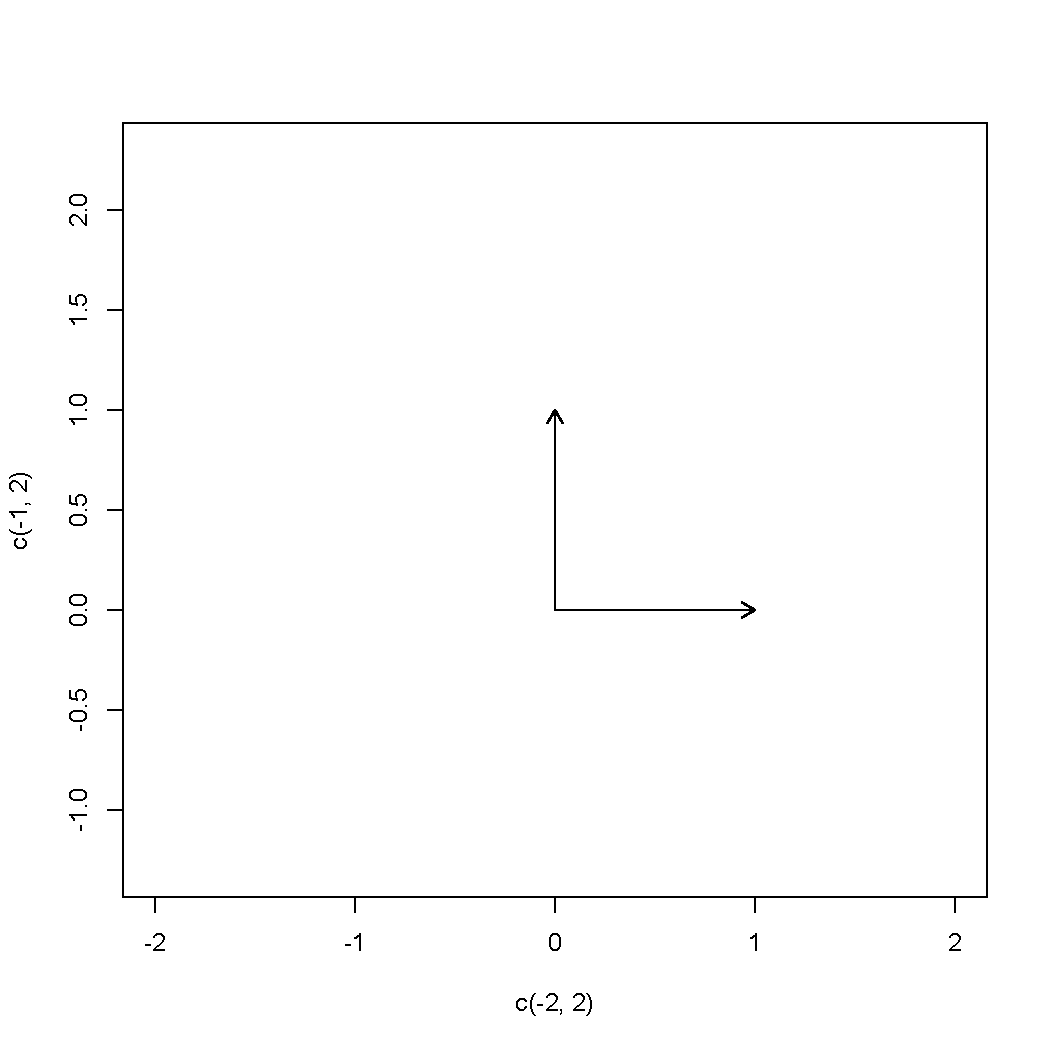
\includegraphics[width=0.33\columnwidth]{./figures/hands-on2/rightangle.pdf}
\caption{A simple vector figure.}
\end{figure}
%
Let's see what the dot product can tell us about these vectors. First recall that we can calculate the length of a vector as the square-root of the dot product of the vector with itself ($\vert\vec{a}\vert^2  =  \vec{a} \cdot \vec{a}$)
\begin{R}
> len.a <- drop(sqrt(a %*% a))
> len.a
[1] 1
> len.b <- drop(sqrt(b %*% b))
\end{R}
%
How about the angle between $a$ and $b$?
\begin{R}
> dot.ab <- a %*% b
> dot.ab
     [,1]
[1,]    0
> cos.ab <- (a %*% b)/(len.a * len.b)
> cos.ab
     [,1]
[1,]    0
\end{R}
A key point to remember dot product of two vectors is zero if, and only if, they are orthogonal to each other (regardless of their dimension).


